\documentclass[dvips, lscape]{foils}
%\documentclass[dvips, french]{slides}
\textwidth 18.5cm
\textheight 25cm 
\topmargin -1cm 
\oddsidemargin  -1cm 
\evensidemargin  -1cm

% Maths
\usepackage{amsfonts, amsmath, amssymb}

\newcommand{\coefbin}[2]{\left( 
    \begin{array}{c} #1 \\ #2 \end{array} 
  \right)}
\newcommand{\bbullet}{\bullet\bullet}
\newcommand{\bbbullet}{\bbullet\bullet}
\newcommand{\bbbbullet}{\bbbullet\bullet}
\newcommand{\Bcal}{\mathcal{B}}
\newcommand{\Ccal}{\mathcal{C}}
\newcommand{\Dcal}{\mathcal{D}}
\newcommand{\Ecal}{\mathcal{E}}
\newcommand{\Mcal}{\mathcal{M}}
\newcommand{\Ncal}{\mathcal{N}}
\newcommand{\Pcal}{\mathcal{P}}
\newcommand{\Qcal}{\mathcal{Q}}
\newcommand{\Lcal}{\mathcal{L}}
\newcommand{\Tcal}{\mathcal{T}}
\newcommand{\Ucal}{\mathcal{U}}
\newcommand{\Xcal}{\mathcal{X}}
\newcommand{\Zcal}{\mathcal{Z}}
\newcommand{\etabar}{\overline{\eta}}
\newcommand{\pibar}{\overline{\pi}}
\newcommand{\alphabf}{\mbox{\mathversion{bold}{$\alpha$}}}
\newcommand{\betabf}{\mbox{\mathversion{bold}{$\beta$}}}
\newcommand{\gammabf}{\mbox{\mathversion{bold}\newcommand{\psibf}{\mbox{\mathversion{bold}{$\psi$}}}
{$\gamma$}}}
\newcommand{\mubf}{\mbox{\mathversion{bold}{$\mu$}}}
\newcommand{\psibf}{\mbox{\mathversion{bold}{$\psi$}}}
\newcommand{\Sigmabf}{\mbox{\mathversion{bold}{$\Sigma$}}}
\newcommand{\taubf}{\mbox{\mathversion{bold}{$\tau$}}}
\newcommand{\thetabf}{\mbox{\mathversion{bold}{$\theta$}}}
\newcommand{\Abf}{{\bf A}}
\newcommand{\Ebf}{{\bf E}}
\newcommand{\Hbf}{{\bf H}}
\newcommand{\Ibf}{{\bf I}}
\newcommand{\Sbf}{{\bf S}}
\newcommand{\mbf}{{\bf m}}
\newcommand{\ubf}{{\bf u}}
\newcommand{\vbf}{{\bf v}}
\newcommand{\xbf}{{\bf x}}
\newcommand{\Xbf}{{\bf X}}
\newcommand{\Esp}{{\mathbb E}}
\newcommand{\Corr}{{\mathbb C}\mbox{orr}}
\newcommand{\Var}{{\mathbb V}}
\newcommand{\Ibb}{{\mathbb I}}
\newcommand{\Rbb}{\mathbb{R}}
\newcommand{\Vsf}{\mathsf{V}}

% Couleur et graphiques
\usepackage{color}
\usepackage{graphics}
\usepackage{epsfig} 
\usepackage{pstcol}

% Texte
\usepackage{lscape}
\usepackage{../../../../Latex/fancyheadings, rotating, enumerate}
%\usepackage[french]{babel}
\usepackage[latin1]{inputenc}
%\definecolor{darkgreen}{cmyk}{0.5, 0, 0.5, 0.5}
%\definecolor{green}{cmyk}{0.5, 0, 0.5, 0.5}
\definecolor{orange}{cmyk}{0, 0.6, 0.8, 0}
\definecolor{jaune}{cmyk}{0, 0.5, 0.5, 0}
\newcommand{\textblue}[1]{\textcolor{blue}{#1}}
\newcommand{\textred}[1]{\textcolor{red}{#1}}
\newcommand{\textgreen}[1]{\textcolor{green}{ #1}}
\newcommand{\textlightgreen}[1]{\textcolor{green}{#1}}
%\newcommand{\textgreen}[1]{\textcolor{darkgreen}{#1}}
\newcommand{\textorange}[1]{\textcolor{orange}{#1}}
\newcommand{\textyellow}[1]{\textcolor{yellow}{#1}}
\newcommand{\refer}[2]{{\sl #1}}

% Sections
%\newcommand{\chapter}[1]{\centerline{\LARGE \textblue{#1}}}
% \newcommand{\section}[1]{\centerline{\Large \textblue{#1}}}
% \newcommand{\subsection}[1]{\noindent{\Large \textblue{#1}}}
% \newcommand{\subsubsection}[1]{\noindent{\large \textblue{#1}}}
% \newcommand{\paragraph}[1]{\noindent {\textblue{#1}}}
% Sectionsred
\newcommand{\chapter}[1]{
  \addtocounter{chapter}{1}
  \setcounter{section}{0}
  \setcounter{subsection}{0}
%  {\centerline{\LARGE \textblue{\arabic{chapter} - #1}}}
  {\centerline{\LARGE \textblue{#1}}}
  }
\newcommand{\section}[1]{
  \addtocounter{section}{1}
  \setcounter{subsection}{0}
%  {\centerline{\Large \textblue{\arabic{chapter}.\arabic{section} - #1}}}
  {\centerline{\Large \textblue{#1}}}
  }
\newcommand{\subsection}[1]{
  \addtocounter{subsection}{1}
%  {\noindent{\large \textblue{\arabic{chapter}.\arabic{section}.\arabic{subsection} - #1}}}
  {\noindent{\large \textblue{#1}}}
  }
\newcommand{\paragraph}[1]{\noindent{\textblue{#1}}}

%%%%%%%%%%%%%%%%%%%%%%%%%%%%%%%%%%%%%%%%%%%%%%%%%%%%%%%%%%%%%%%%%%%%%%
%%%%%%%%%%%%%%%%%%%%%%%%%%%%%%%%%%%%%%%%%%%%%%%%%%%%%%%%%%%%%%%%%%%%%%
%%%%%%%%%%%%%%%%%%%%%%%%%%%%%%%%%%%%%%%%%%%%%%%%%%%%%%%%%%%%%%%%%%%%%%
%%%%%%%%%%%%%%%%%%%%%%%%%%%%%%%%%%%%%%%%%%%%%%%%%%%%%%%%%%%%%%%%%%%%%%
\begin{document}
%%%%%%%%%%%%%%%%%%%%%%%%%%%%%%%%%%%%%%%%%%%%%%%%%%%%%%%%%%%%%%%%%%%%%%
%%%%%%%%%%%%%%%%%%%%%%%%%%%%%%%%%%%%%%%%%%%%%%%%%%%%%%%%%%%%%%%%%%%%%%
%%%%%%%%%%%%%%%%%%%%%%%%%%%%%%%%%%%%%%%%%%%%%%%%%%%%%%%%%%%%%%%%%%%%%%
%%%%%%%%%%%%%%%%%%%%%%%%%%%%%%%%%%%%%%%%%%%%%%%%%%%%%%%%%%%%%%%%%%%%%%
\landscape
\newcounter{chapter}
\newcounter{section}
\newcounter{subsection}
\setcounter{chapter}{0}
\headrulewidth 0pt 
\pagestyle{fancy} 
\cfoot{}
\rfoot{\begin{rotate}{90}{
      \hspace{1cm} \tiny S. Robin: A mixture model for random graphs 
      }\end{rotate}}
\rhead{\begin{rotate}{90}{
      \hspace{-.5cm} \tiny \thepage
      }\end{rotate}}

%%%%%%%%%%%%%%%%%%%%%%%%%%%%%%%%%%%%%%%%%%%%%%%%%%%%%%%%%%%%%%%%%%%%%%
%%%%%%%%%%%%%%%%%%%%%%%%%%%%%%%%%%%%%%%%%%%%%%%%%%%%%%%%%%%%%%%%%%%%%%
\begin{center}
  \textblue{\LARGE A mixture model for random graphs} 

   \vspace{1cm}
   {\large J-J Daudin, F. Picard, \underline{S. Robin}} \\
   robin@inapg.inra.fr

   {UMR INA-PG / ENGREF / INRA, Paris} \\
   {Math�matique et Informatique Appliqu�es}
   
\end{center}

\vspace{2cm}
\paragraph{Examples of networks.} 
$$
\begin{tabular}{ll}
  Social: & who knows who? \\
  \\
  Biological: & which protein interacts with which? \\
  \\
  Internet: & connection between servers or web pages.
\end{tabular}
$$

%%%%%%%%%%%%%%%%%%%%%%%%%%%%%%%%%%%%%%%%%%%%%%%%%%%%%%%%%%%%%%%%%%%%%
%%%%%%%%%%%%%%%%%%%%%%%%%%%%%%%%%%%%%%%%%%%%%%%%%%%%%%%%%%%%%%%%%%%%%
\newpage
\chapter{Random graphs}
%%%%%%%%%%%%%%%%%%%%%%%%%%%%%%%%%%%%%%%%%%%%%%%%%%%%%%%%%%%%%%%%%%%%%

\paragraph{Notation and definition.} Given a set of $n$ vertices ($i = 1..n$),
$X_{ij}$ indicates the presence/absence of a (non oriented) edge
between vertices $i$ and $j$:
$$
X_{ij} = X_{ji} = \Ibb\{i \leftrightarrow j\}, 
\qquad X_{ii} = 0.
$$
The random graph is defined by the join distribution of all the
$\{X_{ij}\}_{i, j}$.

\vspace{1cm}
\paragraph{Typical characteristics.} 

\noindent\begin{tabular}{ll}
  Degree (connectivity) of the vertices: & ${K_i = \sum_{j
      \neq i} X_{ij}}$ \\
  \\
  Clustering coefficient: &  ${c = \Pr\{X_{jk} = 1 \;|\;
    X_{ij} = X_{ik} = 1 \}}$ \\
  \\
  Diameter: & Longest path between two vertices.
\end{tabular}

%%%%%%%%%%%%%%%%%%%%%%%%%%%%%%%%%%%%%%%%%%%%%%%%%%%%%%%%%%%%%%%%%%%%%
\newpage
\subsection{Erdos-R�nyi (ER) model}

\paragraph{Definition.} The $\{X_{ij}\}_{i, j}$ are i.i.d.: 
$$
X_{ij} \sim \Bcal(p).  
$$

\paragraph{Characteristics.}

\noindent\begin{tabular}{ll}
  Degree : & $K_i \sim \Bcal(n-1, p) \approx \Pcal(\lambda)$ \\
  \\
  Clustering coefficient: &  ${c = p}$ \\
\end{tabular}


\vspace{1cm}
\paragraph{Drawback.} The ER fits poorly many real-world networks.
\begin{itemize}
\item Empirical degree distributions are often very different from the
  Poisson distribution because of few vertices having very high
  degrees.
\item Empirical clustering coefficients are generally higher than
  expected under ER.
\end{itemize}

%%%%%%%%%%%%%%%%%%%%%%%%%%%%%%%%%%%%%%%%%%%%%%%%%%%%%%%%%%%%%%%%%%%%%
%%%%%%%%%%%%%%%%%%%%%%%%%%%%%%%%%%%%%%%%%%%%%%%%%%%%%%%%%%%%%%%%%%%%%
\newpage
\chapter{Erd�s-R�nyi mixture for graph (ERMG)} \label{Sec:ErdosMixture}
%%%%%%%%%%%%%%%%%%%%%%%%%%%%%%%%%%%%%%%%%%%%%%%%%%%%%%%%%%%%%%%%%%%%%

%%%%%%%%%%%%%%%%%%%%%%%%%%%%%%%%%%%%%%%%%%%%%%%%%%%%%%%%%%%%%%%%%%%%%
\subsection{An explicit random graph model} 

\paragraph{Mixture population of edges.} We still suppose that the
edges belong to $Q$ groups:
$$
\alpha_q = \Pr\{i \in q\}, 
\qquad
Z_{iq} = \Ibb\{i \in q\}.
$$

\paragraph{Conditional distribution of the edges.}
The edges $\{X_{ij}\}$ are conditionally independent given the group of
the vertices:
$$
X_{ij} \; |\; \{i \in q, j \in \ell \} \sim \Bcal(\pi_{q\ell}).
$$
$\pi_{q\ell} = \pi_{\ell q}$ is the connection probability between
groups $q$ and $\ell$.

A high value of $\pi_{q\ell}$ reveals a preferential connectivity
between groups $q$ and $\ell$. 

%%%%%%%%%%%%%%%%%%%%%%%%%%%%%%%%%%%%%%%%%%%%%%%%%%%%%%%%%%%%%%%%%%%%%
\newpage
\subsection{Some properties of the ERMG model}
%%%%%%%%%%%%%%%%%%%%%%%%%%%%%%%%%%%%%%%%%%%%%%%%%%%%%%%%%%%%%%%%%%%%%

\paragraph{Conditional distribution of the degrees:}
$$
K_i \;|\; \{i \in q \} \sim \Bcal(n-1, \pibar_q) \approx
\Pcal(\lambda_q)
$$
where $ \pibar_q = \sum_{\ell} \alpha_{\ell} \pi_{q\ell}$,
$\lambda_q = (n-1) \pibar_q$.

\bigskip\bigskip
\paragraph{Marginal distribution of the degrees:} we get a Poisson mixture
$$
K_i \sim \sum_q \Bcal(n-1, \pibar_q) \approx \sum_q \alpha_q \Pcal(\lambda_q).
$$

%%%%%%%%%%%%%%%%%%%%%%%%%%%%%%%%%%%%%%%%%%%%%%%%%%%%%%%%%%%%%%%%%%%%%
\newpage
\paragraph{Between-group connectivity.}
$A_{q\ell}$ denotes the connectivity between groups $q$ and $\ell$:
$$
A_{q\ell} = \sum_{i<j} Z_{iq} Z_{j\ell} X_{ij}.
$$
In the ERMG model, its expectation is
$$
\Esp (A_{q\ell})  = \frac{n(n-1)}2 \alpha_q \alpha_{\ell} \pi_{q\ell}.
$$

\paragraph{Clustering coefficient:}  
$$
c = \Pr\{\nabla \cap \Vsf\} / \Pr\{\Vsf\} = \Pr\{\nabla\} /
\Pr\{\Vsf\}.
$$
In the ERMG model, we get
$$
c = \frac{\sum_{q, \ell, m} \alpha_q \alpha_{\ell} \alpha_m \pi_{q\ell}
\pi_{qm} \pi_{\ell m}}{\sum_{q, \ell, m} \alpha_q
  \alpha_{\ell} \alpha_m \pi_{q\ell} \pi_{qm}}.
$$

%%%%%%%%%%%%%%%%%%%%%%%%%%%%%%%%%%%%%%%%%%%%%%%%%%%%%%%%%%%%%%%%%%%%%
\newpage
\subsection{Independent model}
%%%%%%%%%%%%%%%%%%%%%%%%%%%%%%%%%%%%%%%%%%%%%%%%%%%%%%%%%%%%%%%%%%%%%

The absence of preferential connection between groups corresponds to
the case where
$$
\pi_{q\ell} = \eta_q \eta_{\ell}.
$$

\noindent
\begin{tabular}{ll}
  \paragraph{Distribution of degrees:} & $\{K_i \;|\; i \in q\} \sim
  \Pcal(\lambda_q)$, \\
  \\
  & where \quad $\lambda_q = (n-1) \eta_q \etabar$, \quad $\etabar = \sum_{\ell}
  \alpha_{\ell} \eta_{\ell}$. \\
  \\
  \paragraph{Between group connectivity:} & $\Esp (A_{q\ell}) = n(n-1)
  (\alpha_q \eta_q) (\alpha_{\ell} \eta_{\ell}) / 2$. \\
  \\
  \paragraph{Clustering coefficient:} & $\displaystyle{c =  \frac{\left(\sum_q \alpha_q
    \eta^2_q\right)^2}{\etabar^2}}$.
\end{tabular}

The ER model corresponds to 
$$
Q=1, \qquad \alpha_1=1, \qquad \etabar = \eta_1 = \sqrt{p},
$$
so we get the known result: $ c = \eta^4_1 / \eta^2_1 = p $.


%%%%%%%%%%%%%%%%%%%%%%%%%%%%%%%%%%%%%%%%%%%%%%%%%%%%%%%%%%%%%%%%%%%%%
\newpage
\subsection{Examples}
%%%%%%%%%%%%%%%%%%%%%%%%%%%%%%%%%%%%%%%%%%%%%%%%%%%%%%%%%%%%%%%%%%%%%
$$
\begin{tabular}{lcccc}
  Description & Network & $Q$ & $\pi$
  & \begin{tabular}{c} Clustering \\ coefficient \end{tabular}\\
  \hline
  \begin{tabular}{p{2cm}} Random \end{tabular}
  & \begin{tabular}{c}\epsfig{file = ../figures/FigNetworks-Erdos.eps, height=1.7cm,
      width=2.5cm, clip=, bbllx=120, bblly=260, bburx=530,
      bbury=570}  \end{tabular}
  & 1
  &  $p$ & $p$ \\
  \hline
  \begin{tabular}{p{2cm}} Independent model (product connectivity) \end{tabular}
  & \begin{tabular}{c}\epsfig{file = ../figures/FigNetworks-Indep.eps,
      height=2cm, width=4cm, clip=, bbllx=120, bblly=260, bburx=530,
      bbury=570}  \end{tabular}
  & 2
  & $\left( \begin{array}{cc} a^2 &ab\\ ab&b^2\\ \end{array}
  \right)$
  & $\displaystyle{\frac{(a^2+b^2)^2}{(a+b)^2}}$ \\
  \hline
  \begin{tabular}{p{2cm}} Stars \end{tabular}
  & \begin{tabular}{c}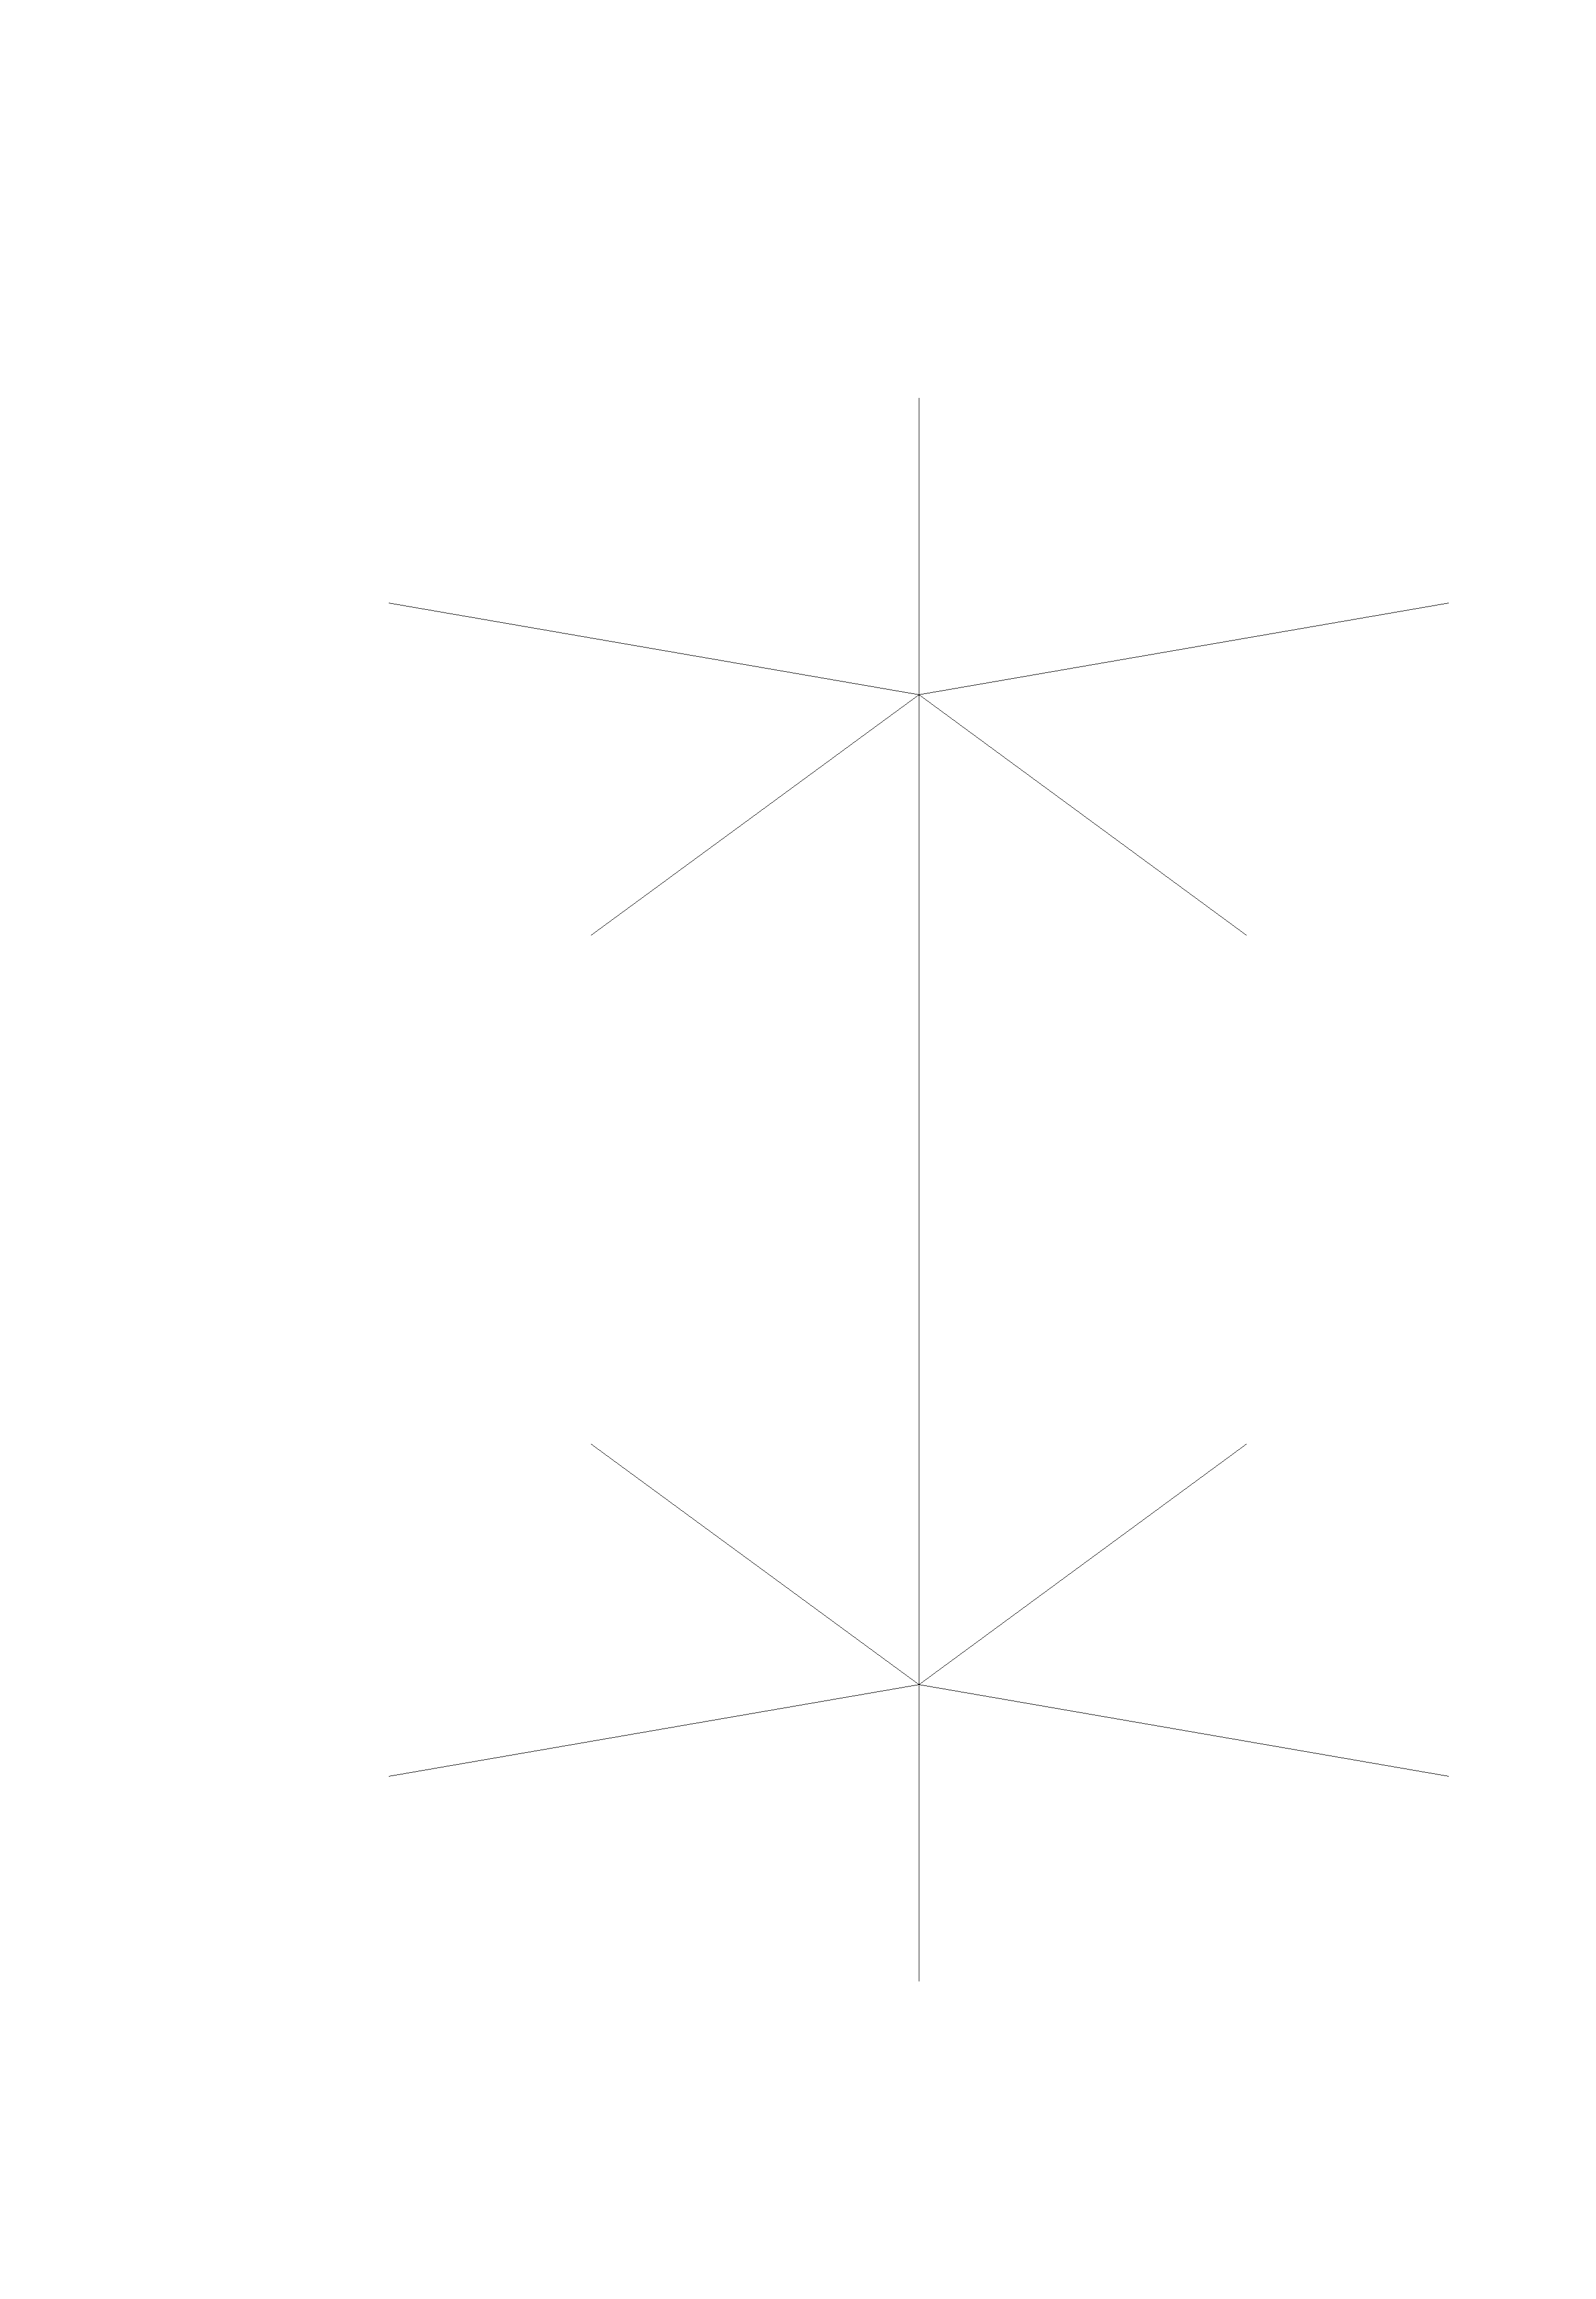
\epsfig{file = ../figures/FigNetworks-Star.eps, height=1.7cm,
      width=4cm, clip=, bbllx=120, bblly=260, bburx=530,
      bbury=570}   \end{tabular}
  & 4
  & $\left( \begin{array}{cccc} 0&1&0&0\\ 1&0&1&0\\0&1&0&1\\0&0&1&0\\
    \end{array} \right)$
  & 0 \\
  \hline \begin{tabular}{p{2cm}} Clusters (affiliation networks)
  \end{tabular}
  
  & \begin{tabular}{c} 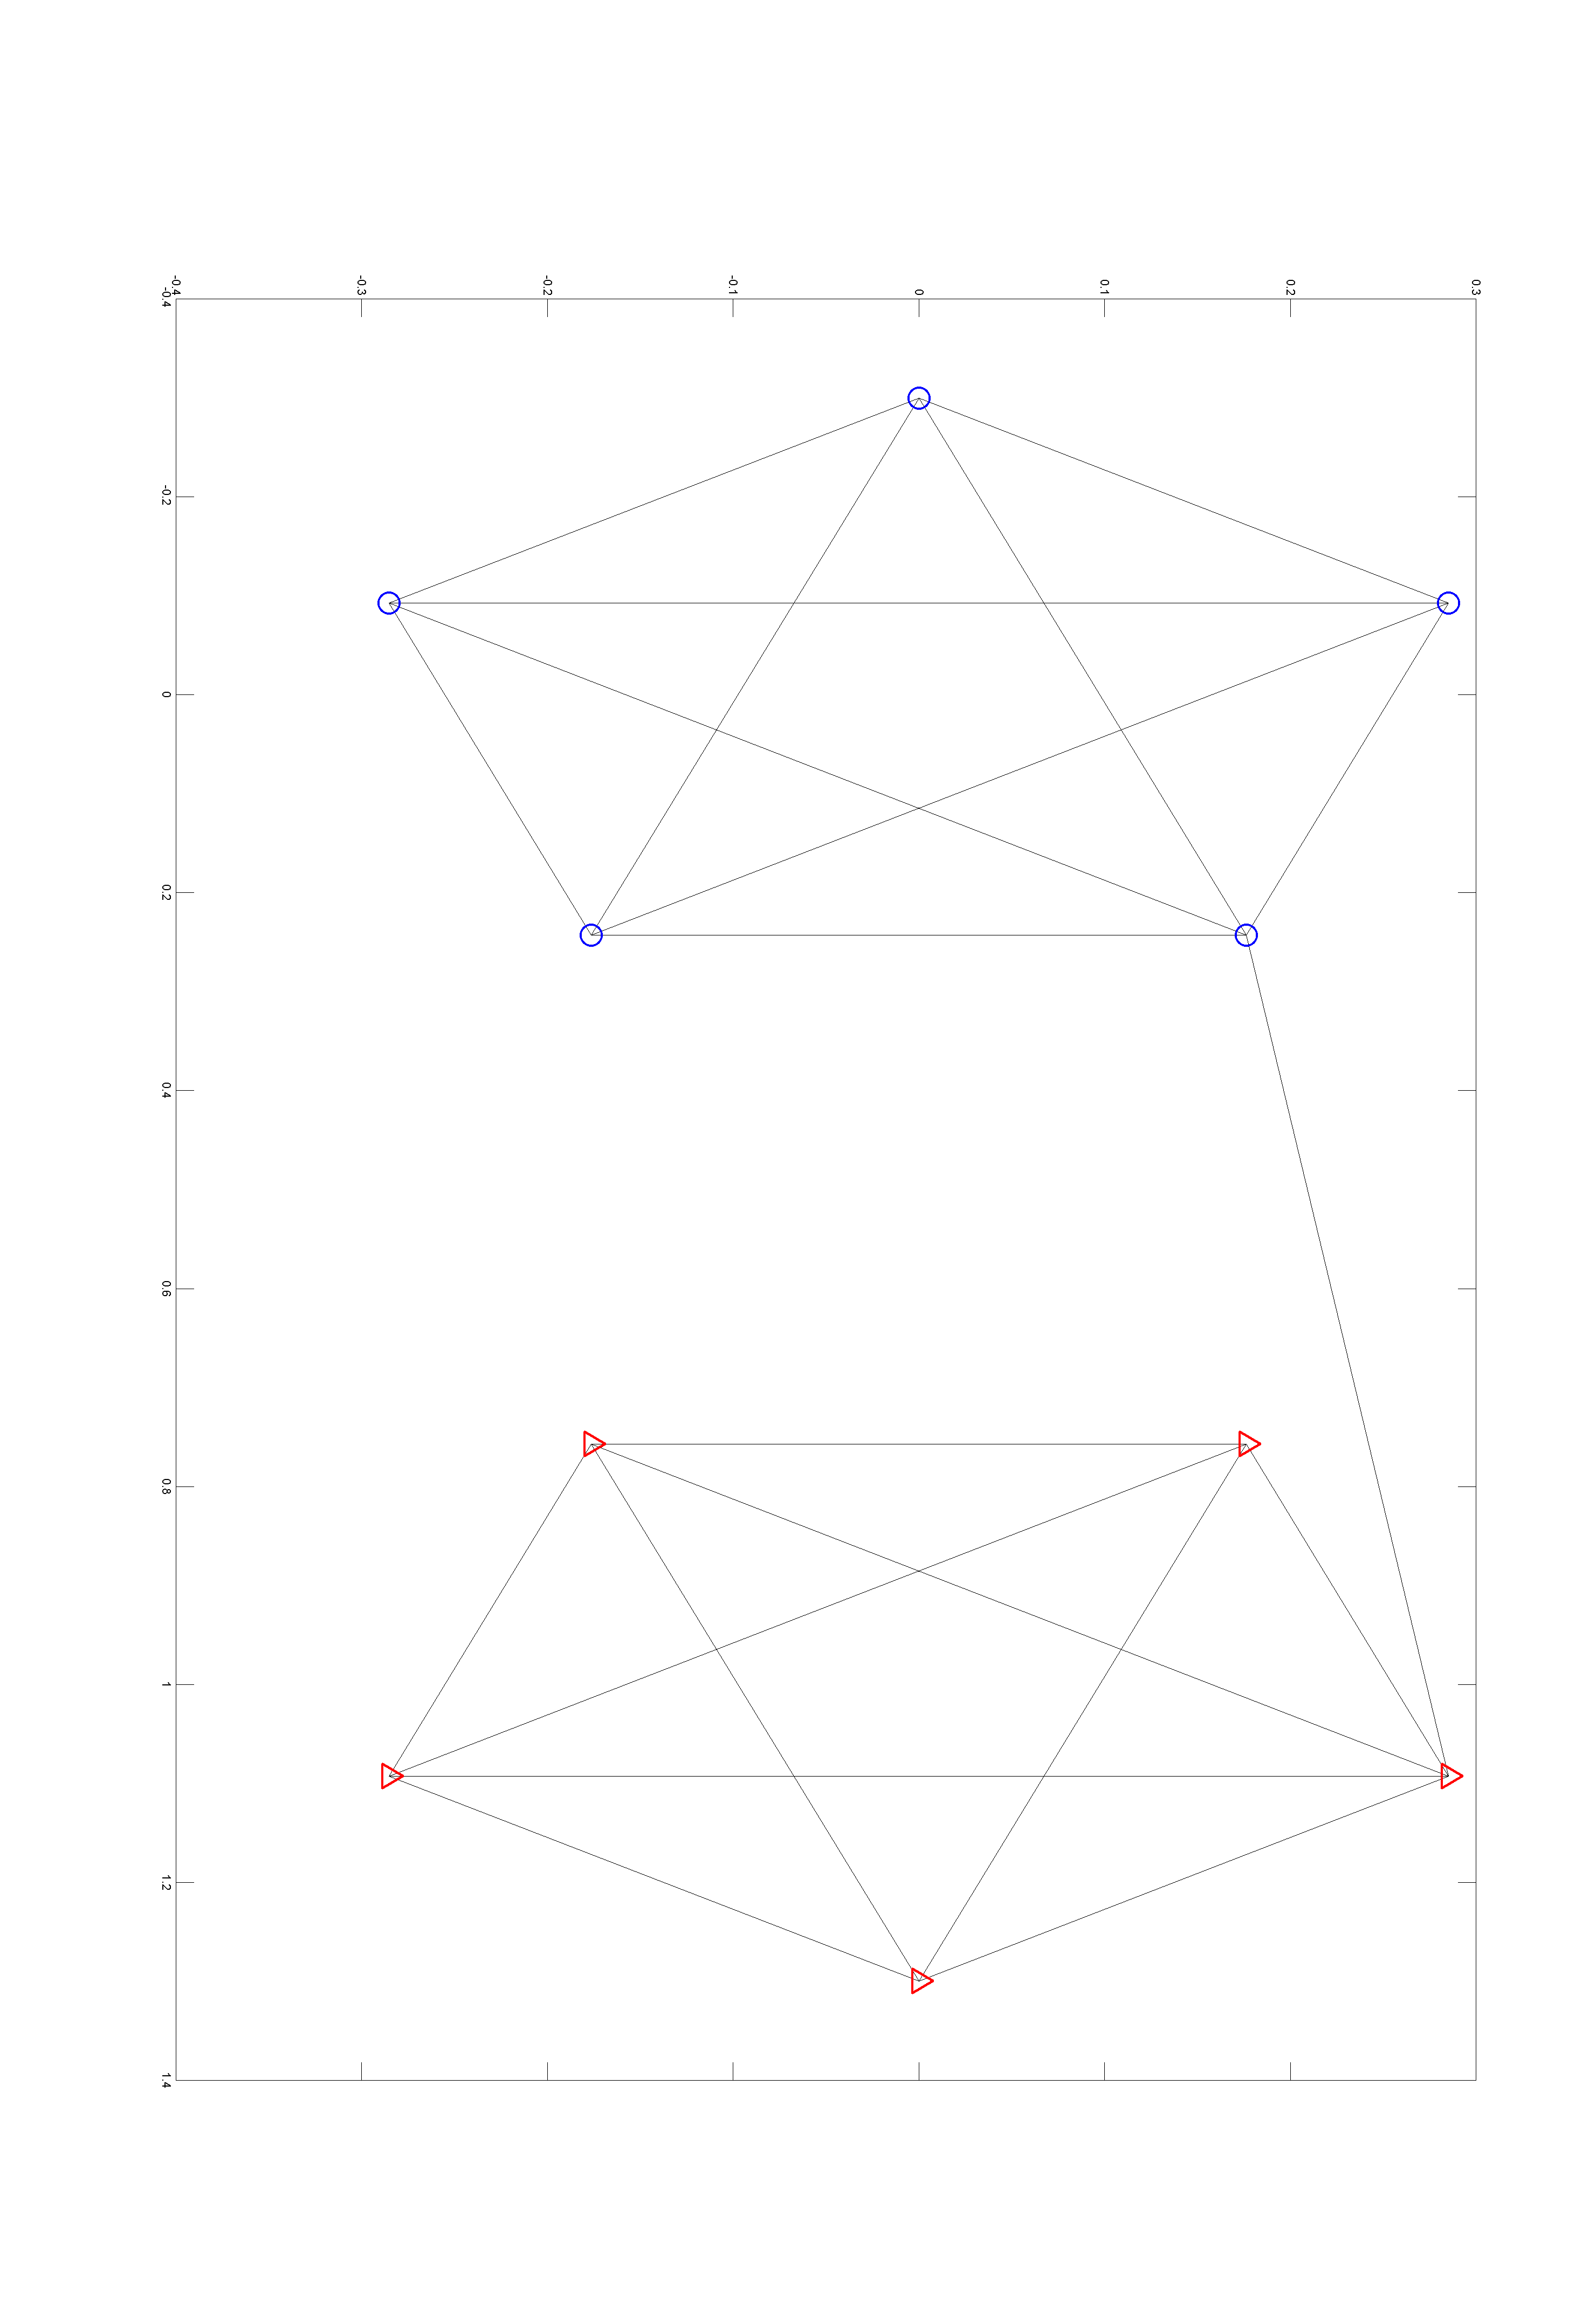
\epsfig{file = ../figures/FigNetworks-Clusters.eps,
      height=1.8cm, width=4cm, clip=, bbllx=120, bblly=260, bburx=530,
      bbury=570}  \end{tabular}
  & 2
  & $\left(\begin{array}{cc} 1&\varepsilon\\ \varepsilon&1\\
    \end{array} \right)$ &
  $\displaystyle{\frac{1+3\varepsilon^2}{(1+\varepsilon)^2}}$ \\ 
\end{tabular}
$$

%%%%%%%%%%%%%%%%%%%%%%%%%%%%%%%%%%%%%%%%%%%%%%%%%%%%%%%%%%%%%%%%%%%%%
\newpage
\paragraph{Scale free network model.}
(Barabasi \& Albert, 99)

The network is build iteratively: the $i$-th vertex joining the
network connects one of the $(i-1)$ preceeding ones with probability
proportional to their current degree (\paragraph{busy gets busier}):
$$
\forall j < i, \qquad \Pr\vspace{0cm}^i\{ i \leftrightarrow j\} \propto K_j^i.
$$
The limit marginal distribution for the degrees is then scale free:
$p(k) \propto k^{-3}$.

\bigskip\bigskip
\paragraph{Analogous modeling with the independent ERMG.} At time $q$,
$n_q = n \alpha_q$ vertices join the net work. They preferentially
connect the oldest vertices:
$$
\pi_{q\ell} = \eta_q \eta_{\ell}, 
\qquad \eta_1 \geq \eta_2 \geq \dots \geq \eta_q \geq \dots 
$$
The decreasing speed of the $\{\eta_q\}$ gives the tail of the degree
distribution. 

%%%%%%%%%%%%%%%%%%%%%%%%%%%%%%%%%%%%%%%%%%%%%%%%%%%%%%%%%%%%%%%%%%%%%
\newpage
\chapter{Maximum likelihood estimation via E-M}
%%%%%%%%%%%%%%%%%%%%%%%%%%%%%%%%%%%%%%%%%%%%%%%%%%%%%%%%%%%%%%%%%%%%%

We denote $\Xcal = \{X_{ij}\}_{i, j = 1..n}$, $\Zcal=
\{Z_{iq}\}_{i=1..n, q=1..Q}$.

%%%%%%%%%%%%%%%%%%%%%%%%%%%%%%%%%%%%%%%%%%%%%%%%%%%%%%%%%%%%%%%%%%%%%
\subsection{Likelihood}
%%%%%%%%%%%%%%%%%%%%%%%%%%%%%%%%%%%%%%%%%%%%%%%%%%%%%%%%%%%%%%%%%%%%%

The conditional expectation of the complete-data log-likelihood is
\begin{eqnarray*}
  \Qcal(\Xcal) &=& \Esp \left\{ \Lcal(\Xcal,\Zcal)|\Xcal \right\}  \\
  \\
  &=&  \sum_i \sum_q \tau_{iq} \log \alpha_q
  + \sum_i \sum_q \sum_{j > i} \sum_{\ell} \theta_{ijq\ell} \log
  b(X_{ij}; \pi_{q\ell}),
\end{eqnarray*}
where $\tau_{iq}$ and $\theta_{ijq\ell}$ are {\sl posterior}
probabilities
$$
\tau_{iq} = \Pr\{Z_{iq} = 1 \;|\; \Xcal\}, \qquad
\theta_{ijq\ell} = \Pr\{Z_{iq} Z_{j\ell} = 1 \;|\; \Xcal\}
$$
% \begin{eqnarray*}
%   \tau_{iq} & = & \Pr\{Z_{iq} = 1 \;|\; \Xcal\} = \Esp(Z_{iq} \;|\;
%   \Xcal), \\
%   \\
%   \theta_{ijq\ell} & = & \Pr\{Z_{iq} Z_{j\ell} = 1 \;|\; \Xcal\} =
%   \Esp(Z_{iq} Z_{j\ell} \;|\; \Xcal). 
% \end{eqnarray*}
Evaluating these probabilities is not straightforward because the
$\{Z_{iq}\}$ are all dependent conditionally on $\Xcal$.

%%%%%%%%%%%%%%%%%%%%%%%%%%%%%%%%%%%%%%%%%%%%%%%%%%%%%%%%%%%%%%%%%%%%%
\newpage
\paragraph{E step.}
We approximate the conditional joint distribution of the $\{Z_{iq}\}$:
\begin{eqnarray*}
  \Pr\{\Zcal \;|\; \Xcal\} & \simeq & \prod_i \Pr\{\Zcal_i \;|\; \Xcal,
  \Zcal^i\} \\
  \quad \mbox{where} \quad
  \Pr\{Z_{iq} = 1 \;|\; \Xcal, \Zcal^i\} & \propto & \alpha_q \prod_{m}
  b(C_{im}; N^i_{m} , \pi_{qm})
\end{eqnarray*}
\begin{itemize}
\item The elements of $\Zcal^i$ are estimated by their conditional
  expectation: $ \widehat{Z}_{j\ell} = \tau_{j\ell}$.
\item The posterior probabilities $\tau_{iq}$ must therefore satisfy 
  $$
  \widehat{\tau}_{iq} = \Pr\{Z_{iq} = 1 \;|\; \Xcal,
  \widehat{\Zcal}^i\} 
  $$
  which is actually a fix point type relation.  The
  $\widehat{\tau}_{iq}$ are obtained by iterating it.
\end{itemize}

\paragraph{M step.}
Maximizing $\Qcal(\Xcal)$ subject to $\sum_q \alpha_q = 1$ gives
$$
\widehat{\alpha}_q = \sum_i \widehat{\tau}_{iq} / n, \qquad
\widehat{\pi}_{q\ell} = \sum_i \sum_j \widehat{\theta}_{ijq\ell}
X_{ij} \left/ \sum_i \sum_j \widehat{\theta}_{ijq\ell} \right..
$$

%%%%%%%%%%%%%%%%%%%%%%%%%%%%%%%%%%%%%%%%%%%%%%%%%%%%%%%%%%%%%%%%%%%%%
\newpage
\subsection{Choice of the number of groups}
%%%%%%%%%%%%%%%%%%%%%%%%%%%%%%%%%%%%%%%%%%%%%%%%%%%%%%%%%%%%%%%%%%%%%

We propose a heuristic penalized likelihood criterion inspired from
BIC.

Since $\Qcal(\Xcal)$ is the sum of
$$
\begin{tabular}{p{11cm}p{13cm}}
  $\displaystyle{\sum_i \sum_q \tau_{iq} \log \alpha_q}$ & 
  which deals with $(Q-1)$ independent proportions $\alpha_q$s and
  involves $n$ terms, 
  \\ 
  \\
  $\displaystyle{\sum_i \sum_q \sum_{j > i} \sum_{\ell} \theta_{ijq\ell} \log
    b(X_{ij}; \pi_{q\ell})}$ 
  & which deals with $Q(Q+1)/2$ probabilities $\pi_{q\ell}$s and
  involves $n(n-1)/2$ terms,
\end{tabular}
$$
we propose the following heuristic criterion:
$$
- 2\Qcal(\Xcal) + (Q-1) \log n + \frac{Q(Q+1)}2
\log\left[\frac{n(n-1)}2\right].
$$

%%%%%%%%%%%%%%%%%%%%%%%%%%%%%%%%%%%%%%%%%%%%%%%%%%%%%%%%%%%%%%%%%%%%%
\newpage
\chapter{Application to Karate Club Data}
%%%%%%%%%%%%%%%%%%%%%%%%%%%%%%%%%%%%%%%%%%%%%%%%%%%%%%%%%%%%%%%%%%%%%

\begin{itemize}
\item \vspace{-0.5cm} $n = 34$ members (vertices) of a Karate club
\item \vspace{-0.5cm} 2 members are connected is they have social
  interactions (apart from their sportive activity)
\item \vspace{-0.5cm} $156$ edges.
\end{itemize}
\vspace{-0.5cm}
This dataset (Zachary, 77) has been intensively studied in the
literature, generally with $Q = 4$ groups.

\paragraph{Parameter estimates.}
$$
\vspace{-1cm}
\begin{array}{ccccc}
  \widehat{\alpha} (\%) & 5.9 & 8.9 & 36.8 & 48.4 \\
  \hline
  & 100 & 16.5 & 6.8 & 73.8 \\
  \widehat{\pi} & 16.5 & 100 & 52.9 & 16.0 \\
  (\%) & 6.8 & 52.8 & 12.3 & 0.0 \\
  & 73.8 & 16.0 & 0.0 & 7.8 \\
  \hline
  \widehat{\lambda} & 15.0 & 12.2 & 3.2 & 3.2
\end{array}
$$

\paragraph{Clustering coefficient.}
ERMG models gives $0.314$ while the empirical $c$ is $0.256$.

%%%%%%%%%%%%%%%%%%%%%%%%%%%%%%%%%%%%%%%%%%%%%%%%%%%%%%%%%%%%%%%%%%%%%
\newpage
\hspace{-2cm}
\begin{tabular}{cc}
  \begin{tabular}{p{11cm}}
    \paragraph{Dot-plot representation of the graph.} \\ \\
    Dot present means 
    $$X_{ij} = 1$$
    The vertices are re-ordered according to their 'mean group
    number':
    $$
    \widehat{q}_i = \sum_q q \; \widehat{\tau}_{iq} 
    $$
  \end{tabular}
  &
  \begin{tabular}{c}
    \epsfig{file = ../figures/Karate-ERMG-Ward-Q4_class.eps,
      height=13cm, width=13cm, clip=,bbllx=70, bblly=440, bburx=540,
      bbury=770}   
  \end{tabular} 
  \vspace{-1cm}
  \\
  \begin{tabular}{p{11cm}}
    \paragraph{Posterior probabilities $\widehat{\tau}_{iq}$.}  \\ \\ \\
  \end{tabular}
  & 
  \begin{tabular}{c}
    \epsfig{file = ../figures/Karate-ERMG-Ward-Q4_class.eps,
    width=13cm, clip=, bbllx=70, bblly=265, bburx=540, bbury=420}  
  \end{tabular}
\end{tabular}

%%%%%%%%%%%%%%%%%%%%%%%%%%%%%%%%%%%%%%%%%%%%%%%%%%%%%%%%%%%%%%%%%%%%%
\newpage
\paragraph{Interpretation of the groups}
\begin{itemize}
\item 2 persons, including the administrator, strongly connected with
  group 4, but not with groups 2 and 3;
\item 3 persons including the instructor, strongly connected with
  group 3, but not with groups 1 and 4;
\item 13 'ordinary' members, connected with the instructor;
\item 16 'ordinary' members, connected with the administrator.
\end{itemize}

\paragraph{End of the story.}
The instructor (group 2) finally leaved the club and started another
one with about one half the members (corresponding to group 3?).

%%%%%%%%%%%%%%%%%%%%%%%%%%%%%%%%%%%%%%%%%%%%%%%%%%%%%%%%%%%%%%%%%%%%%
\newpage
\hspace{-2cm}
\begin{tabular}{cc}
  \begin{tabular}{p{11cm}}
    \paragraph{Selection of the number of groups.}  \\ 
    The pseudo BIC actually selects $Q=6$ groups \\ \\ 
    \paragraph{Comparison with the 4 group model.} \\ 
    Former groups 1 and 4 are conserved. \\
    Former groups 2 and 3 are each divided in two new groups \\ \\ 
    We do not know if the new club did last very long... \\ \\ \\ 
  \end{tabular}
  &
  \begin{tabular}{c}
    \epsfig{file = ../figures/Karate-ERMG-Ward-Q6_class.eps,
      height=13cm, width=13cm, clip=,bbllx=70, bblly=440, bburx=540,
      bbury=770}   
  \end{tabular} 
  \vspace{-1cm}
  \\
  \begin{tabular}{p{11cm}}
    \paragraph{Posterior probabilities $\widehat{\tau}_{iq}$.}  \\ \\
  \\ \\  \end{tabular}
  & 
  \begin{tabular}{c}
    \epsfig{file = ../figures/Karate-ERMG-Ward-Q6_class.eps,
    width=13cm, clip=, bbllx=70, bblly=265, bburx=540, bbury=420}  
  \end{tabular}
\end{tabular}


%%%%%%%%%%%%%%%%%%%%%%%%%%%%%%%%%%%%%%%%%%%%%%%%%%%%%%%%%%%%%%%%%%%%%
\newpage
\chapter{Application to {\sl E. coli} reaction network}
%%%%%%%%%%%%%%%%%%%%%%%%%%%%%%%%%%%%%%%%%%%%%%%%%%%%%%%%%%%%%%%%%%%%%
\begin{itemize}
\item \vspace{-0.5cm} $n = 605$ vertices (reactions) and $1\;782$
  edges. 
\item \vspace{-0.5cm} 2 reactions $i$ and $j$ are connected if the
  product of $i$ is the substrate of $j$ (or conversely).
\item \vspace{-0.5cm} provided by V. Lacroix and M.-F. Sagot (INRIA
H�lix).
\end{itemize}

\vspace{-.5cm}
\paragraph{Number of groups.} Pseudo-BIC selects $Q = 21$.

\paragraph{Group proportions.} $\widehat{\alpha}_q$ (\%).
$$
\vspace{-.5cm}
\epsfig{file = ../figures/Ecoli-Complet-ERMG-Ward-Q21_param.eps, height=6cm,
  width=12cm, clip=, bbllx=75, bblly=570, bburx=530, bbury=770}  
$$
\vspace{-.5cm}
Many small groups actually correspond to cliques or pseudo-cliques.

%%%%%%%%%%%%%%%%%%%%%%%%%%%%%%%%%%%%%%%%%%%%%%%%%%%%%%%%%%%%%%%%%%%%%
\newpage
\hspace{-2cm}
\begin{tabular}{cc}
  \begin{tabular}{p{11cm}}
    \paragraph{Dot-plot representation of the graph.} \\ \\ \\
    \paragraph{Biological interpretation:} Groups 1 to 20 gather
    reactions involving all the  same compound either as a substrate or as a
    product. \\ \\
    A compound (pyruvate, ATP, {\sl etc}) can be associated to each
    group. \\ \\ \\
  \end{tabular}
  &
  \begin{tabular}{c}
    \epsfig{file = ../figures/Ecoli-Complet-ERMG-Ward-Q21_class.eps,
      height=13cm, width=13cm, clip=,bbllx=70, bblly=440, bburx=540,
      bbury=770}   
  \end{tabular} 
  \vspace{-1cm}
  \\
  \begin{tabular}{p{11cm}}
    \paragraph{Posterior probabilities $\widehat{\tau}_{iq}$.}  \\ \\ \\
  \end{tabular}
  & 
  \begin{tabular}{c}
    \epsfig{file = ../figures/Ecoli-Complet-ERMG-Ward-Q21_class.eps,
    width=13cm, clip=, bbllx=70, bblly=265, bburx=540, bbury=420}  
  \end{tabular}
\end{tabular}
%$$

%%%%%%%%%%%%%%%%%%%%%%%%%%%%%%%%%%%%%%%%%%%%%%%%%%%%%%%%%%%%%%%%%%%%%
\newpage
\hspace{-2cm}
\begin{tabular}{cc}
  \begin{tabular}{p{9cm}}
    \paragraph{Zoom (bottom left).} \\ 
    \\
    Submatrix of $\pi$:
    $$
    \begin{tabular}{c|cccc}
      $q, \ell$ & 1 & 9 & 10 & 16 \\
      \hline 
      1 & \paragraph{\bf 1.0} \\ 
      9 & \paragraph{\sl .11} & .65 \\ 
      10 & \paragraph{\sl .43} & & .67  \\ 
      16 & \paragraph{\bf 1.0} & \paragraph{\sl .01} & & \paragraph{\bf 1.0} \\ 
    \end{tabular}
    $$
    \\ \\ 
  \end{tabular}
  &
  \begin{tabular}{l}
    \hspace{1.3cm}
    \epsfig{file = ../figures/Ecoli-Complet-ERMG-Ward-Q21_class.eps,
      height=12cm, width=12cm, clip=,bbllx=90, bblly=485, bburx=277,
      bbury=605.5}   
  \end{tabular}  
  \vspace{-2cm}
  \\ \\ \\
  \begin{tabular}{p{9cm}}
    \paragraph{Vertices degree $K_i$.}  \\ \\ 
    Mean degree in the last group:\\ 
    $\overline{K}_{21} = 2.6$ \\ \\ \\
  \end{tabular}
  & 
  \begin{tabular}{l}
    \epsfig{file = ../figures/Ecoli-Complet-ERMG-Ward-Q21_class.eps,
    width=13.4cm, height=6cm, clip=, bbllx=70, bblly=105, bburx=277,
    bbury=245}   
  \end{tabular}
\end{tabular}

%%%%%%%%%%%%%%%%%%%%%%%%%%%%%%%%%%%%%%%%%%%%%%%%%%%%%%%%%%%%%%%%%%%%%
\newpage
%\hspace{-2cm}
% \begin{tabular}{ll}
%   \begin{tabular}{p{11cm}}
%     \paragraph{Between group connectivity.} \\
%     Observed vs predicted: quite good \\ \\ 
%     but the 'observed' $A_{q\ell}$ are not observed but estimated with the MAP
%     rule:
%     $$
%     {\widehat{A}_{q\ell} = \sum_{i<j} \widehat{Z}_{iq}
%       \widehat{Z}_{j\ell} X_{ij}}
%     $$
%     so the observed good fit is optimistic. \\ \\ \\
%   \end{tabular}
%   & 
%   \begin{tabular}{c}
%     \epsfig{file =
%       ../figures/Ecoli-Complet-ERMG-Ward-Q21_param.eps, height=10cm,
%       width=10cm, clip=, bbllx=70, bblly=300, bburx=530, bbury=530}   
%   \end{tabular}
% \end{tabular}
\paragraph{Distribution of the degree.} According to the ERMG, de
      degrees have a Poisson mixture distribution.
$$
\vspace{-1cm}
\begin{tabular}{cc}
  Histogram + mixture distribution & P-P plot \\
  \multicolumn{2}{c}{
    \epsfig{file =
      ../figures/Ecoli-Complet-ERMG-Ward-Q21_degree.eps, height=8cm,
      width=20cm, clip=, bbllx=80, bblly=210, bburx=550, bbury=590}   
    }
\end{tabular}
$$

\paragraph{Clustering coefficient.}
$$
\begin{tabular}{cccc}
  Empirical & ERMG ($Q = 6$) & ERMG ($Q = 21$) & ER ($Q = 1$)\\
  \hline
  0.626 & 0.436 & 0.544 & 0.0098
\end{tabular}
$$

%%%%%%%%%%%%%%%%%%%%%%%%%%%%%%%%%%%%%%%%%%%%%%%%%%%%%%%%%%%%%%%%%%%%%%%%
\newpage
%$$
\vspace{-2cm}
\hspace{-2cm}
\begin{tabular}{cc}
  \begin{tabular}{l}
    \paragraph{Reaction graph.} \\ \\ 
    Group number \\
    (group size) \\ \\ \\ \\ \\ \\ \\ \\ \\ \\ \\ \\ \\ \\ \\ 
  \end{tabular}
  &
  \begin{tabular}{l}
    \epsfig{file = ../figures/Ecoli-Complet-ERMG-Ward-Q21_graph.eps, height=18cm,
      width=18cm, clip=, bbllx=130, bblly=170, bburx=500, bbury=700} 
  \end{tabular}
\end{tabular}
%$$

%%%%%%%%%%%%%%%%%%%%%%%%%%%%%%%%%%%%%%%%%%%%%%%%%%%%%%%%%%%%%%%%%%%%%%%%
\newpage
\chapter{Conclusions}

\paragraph{Past.} 
\begin{itemize}
\item \vspace{-0.5cm} The ERMG model is a flexible generalization of
  the ER model and a promising alternative to the scale-free 'model'.
\item \vspace{-0.5cm} It seems to fit well several real-world networks
  %(Airport network, Enzyme network in bacteria, etc.).
\item \vspace{-0.5cm} It is properly defined, so its properties can be
  properly studied.
\end{itemize}

\paragraph{Future.}
\begin{itemize}
\item \vspace{-0.5cm} Study the probabilistic properties of the ERMG
  model (diameter, probability for a subgraph to be connected, etc).
\item \vspace{-0.5cm} Derive a relevant criterion to select the number
  of groups.
\item \vspace{-0.5cm} Extension to valued graphs: $X_{ij}$ not only
  0/1, but some measure of the connection intensity.
\end{itemize}

% %%%%%%%%%%%%%%%%%%%%%%%%%%%%%%%%%%%%%%%%%%%%%%%%%%%%%%%%%%%%%%%%%%%%%%%%
% \newpage

% \paragraph{Estimated connection probabilities $\pi_{q\ell}$.} (\%)\\
% %$$
% ${\footnotesize
%   \hspace{-2.5cm}
%   \begin{array}{c|ccccccccccccccccccccc}
% & 1 & 2 & 3 & 4 & 5 & 6 & 7 & 8 & 9 & 10 & 11 & 12 & 13 & 14 & 15 & 16 & 17 & 18 & 19 & 20 & 21 \\ 
% \hline 
% 1 & 100 & & & & & & & & & & & & & & & & & & & &  \\ 
% 2 & & 100 & & & & & & & & & & & & & & & & & & &  \\ 
% 3 & & & 100 & & & & & & & & & & & & & & & & & &  \\ 
% 4 & & & & 71 & & & & & & & & & & & & & & & & &  \\ 
% 5 & & & & & 100 & & & & & & & & & & & & & & & &  \\ 
% 6 & & & & & 28 & 100 & & & & & & & & & & & & & & &  \\ 
% 7 & 64 & & & & & & 58 & & & & & & & & & & & & & &  \\ 
% 8 & & & & & & & & 63 & & & & & & & & & & & & &  \\ 
% 9 & 11 & & & & & & 10 & & 65 & & & & & & & & & & & &  \\ 
% 10 & 43 & & & & 1 & & 4 & & & 67 & & & & & & & & & & &  \\ 
% 11 & & & & & & & & & & & 62 & & & & & & & & & &  \\ 
% 12 & & & 4 & & & & 7 & 5 & & & & 28 & & & & & & & & &  \\ 
% 13 & 2 & & 7 & & & & 5 & & & 1 & & 5 & 100 & & & & & & & &  \\ 
% 14 & & & & & & 6 & & & & & 7 & & & 25 & & & & & & &  \\ 
% 15 & & & 1 & & & & & & & & & & & & 40 & & & & & &  \\ 
% 16 & 100 & & & & 18 & & 5 & & 1 & & & 5 & 1 & & & 100 & & & & &  \\ 
% 17 & & & & & & & & & 2 & & 4 & & & & & & 100 & & & &  \\ 
% 18 & & & 1 & & & & & 3 & 2 & & & & & & & & & 21 & & &  \\ 
% 19 & & & & & 16 & & & & & & & & & & & & 0 & & 19 & &  \\ 
% 20 & & & & & & & & & & & & & & & 0 & & 6 & & 0 & 11 &  \\ 
% 21 & & 0 & 0 & 0 & 0 & 0 & 0 & 0 & 0 & 0 & 0 & 0 & 0 & 0 & 0 & 0 & 0 & 0 & 0 & 0 & 1  \\ 
%   \end{array}
% }$
% %$$

%%%%%%%%%%%%%%%%%%%%%%%%%%%%%%%%%%%%%%%%%%%%%%%%%%%%%%%%%%%%%%%%%%%%%%%%
%%%%%%%%%%%%%%%%%%%%%%%%%%%%%%%%%%%%%%%%%%%%%%%%%%%%%%%%%%%%%%%%%%%%%%%%
%%%%%%%%%%%%%%%%%%%%%%%%%%%%%%%%%%%%%%%%%%%%%%%%%%%%%%%%%%%%%%%%%%%%%%%%
%%%%%%%%%%%%%%%%%%%%%%%%%%%%%%%%%%%%%%%%%%%%%%%%%%%%%%%%%%%%%%%%%%%%%%%%
\end{document}
%%%%%%%%%%%%%%%%%%%%%%%%%%%%%%%%%%%%%%%%%%%%%%%%%%%%%%%%%%%%%%%%%%%%%%%%
%%%%%%%%%%%%%%%%%%%%%%%%%%%%%%%%%%%%%%%%%%%%%%%%%%%%%%%%%%%%%%%%%%%%%%%%
%%%%%%%%%%%%%%%%%%%%%%%%%%%%%%%%%%%%%%%%%%%%%%%%%%%%%%%%%%%%%%%%%%%%%%%%
%%%%%%%%%%%%%%%%%%%%%%%%%%%%%%%%%%%%%%%%%%%%%%%%%%%%%%%%%%%%%%%%%%%%%%%%

